\subsection{Finite reflection templates}
\label{calc:reflection-construction}

We construct finitely many reflections that place nearly the full
weighted inventory of each probe in a clear diagonal extraction slab.
This is the geometric input to the mixed-stencil estimate in
Section~\ref{obs:mixed-section}. Horizontal folds create long runs of
repeated cells along the vertical coordinate around the probes; vertical folds align most probe
columns so that their slope-$+1$ lines pass through the gaps in every
vertical wall. A finite extraction tree then removes those probes.

All expected counts below use the half-weights of a binary tree of
inequalities, rather than a law of lattice configurations. The geometry
is independent of the random-cluster parameter. Its extraction
operations use Proposition~\ref{prop:finite-extraction};
Corollary~\ref{cor:finite-extraction-rates} supplies the corresponding
physical norm inequalities when the template is applied to the
observable. Iterating those inequalities averages the extraction
exponents with these same half-weights. The expected counts below
record the extracted probe exponents and give expected copy count one
for each original background feature; after a preliminary fold, its
expected even and odd counts are both $1/2$.
Section~\ref{obs:mixed-section} separately estimates the remaining leaf
norms, bounding their logarithmic background costs by fixed contributions
indexed by the original feature and its reflection parity, together with
controlled remainder terms.
Only after those estimates are the copy-count identities used to average
the costs.

\paragraph{The geometric data.}
Work in the orthogonal tile coordinates $(x,y)$. The data consist of
finitely many initial horizontal and vertical solid segments, marked
features on them, remote endpoints, and two distinct interior probe points
$v_i=(x_i,y_i)$, $i=1,2$. Small local insertion boxes will surround the
probes. The true vertical wall levels lie in
\[
 X_*+G_*\Z,\qquad G_*>0.
\]
This is the only arithmetic property of the rational polygon that
we use. The two probe ordinates are distinct, avoid all horizontal
walls and feature heights, and lie in disjoint open bands containing
no remote endpoint. Their abscissas avoid the vertical wall levels.
Finally, the probes lie on neither of the same two axis diagonals:
\[
 x_1-y_1\ne x_2-y_2,
 \qquad x_1+y_1\ne x_2+y_2.
\]
All these conditions have strict margins on a sufficiently small
compact product neighborhood of the probe pair. We call such a
neighborhood \emph{eligible}.  The forbidden wall levels and feature
heights here refer to these initial data, before any probe-dependent
primary anchors, secondary gaps, or cut locations are chosen.  The
latter enter each finite template, not the global exceptional set.

For a tensor-diagram application, fix the common diagonal routes so
that each probe box meets only its own arriving prefix. All other
diagonal chains avoid both boxes. Shrinking the eligible neighborhood
preserves this condition for every stencil term. Subsequent joins and
reroutings are required to preserve these intact boxes; the proof
below verifies this invariant through the entire template.

Open primary gaps at every true corner. For each probe neighborhood,
choose a fixed anchor ordinate $y_{*,i}$ and a number $H_i>0$ such that
$G_*/(2H_i)$ is a positive integer. Shrink the neighborhoods, and
choose $H_i$ small compared with their distances to other feature
heights and with the larger of the two horizontal clearances at the
probe. Require that, for every $y_i$ in its neighborhood,
\begin{equation}
 l_i=\frac{y_i+y_{*,i}-H_i}{2},\qquad
 y_i\in(l_i,l_i+H_i),
 \qquad 2l_i+H_i=y_i+y_{*,i},
 \label{calc:marker-cell}
\end{equation}
with uniform positive margins. Both intervals in
\eqref{calc:marker-cell} lie in their respective feature-free bands.
This is possible by taking $y_{*,i}$ at the center of the probe band,
then taking its width smaller than $H_i$. Open a primary gap centered
at $y_{*,i}$ on every vertical wall that meets that band. The primary
gaps have fixed positive widths, comparable to a sufficiently small
$h$; they avoid the marked features and one another. Their widths
remain fixed throughout the construction below.

A \emph{fold} across an axis-parallel line retains either open
half-plane and adjoins its reflected copy. Each of the two resulting
diagrams has exponent $1/2$ in the Cauchy--Schwarz inequality. A cut
will eventually be made vacant by small secondary gaps, if necessary.
It never meets a probe box, marked feature, or remote endpoint. A
copy of a probe is \emph{favorable} if the slope-$+1$ line through it
has a solid-free open slab of positive width, containing no other
local insertion or endpoint and no marked feature. We also require
that the values $x-y$ of all the insertion copies in the diagram are
distinct. The widths and separations here are macroscopic constants;
they need not be uniform as $h$ tends to zero.

For a finite binary tree, assign a leaf the product of the factors
$1/2$ on its ancestral edges. An \emph{expected count} always means
the sum of its leaf counts with these weights. Tag each probe and
each retained feature by its original identity, so that copies can
be counted separately for every original object.
For the feature ledger, the original diagram is understood after
all primary and secondary gaps have been inserted: its solid
features are the resulting separated straight fragments and their
tips, together with the protected marks and endpoints. A segment
that is later divided by a secondary gap is not counted as one
intact feature across that gap.

\begin{lemma}[Finite reflection templates]
\label{lem:reflection-templates}
Fix eligible geometric data and their primary gaps. For every
$\varepsilon>0$, there is a finite tree of axis folds and
extraction operations satisfying the finite hypotheses of
Proposition~\ref{prop:finite-extraction}, together
with finitely many secondary gaps on the remaining straight solids,
such that the expected extracted count of each original probe is at
least $1-\varepsilon$. Every cut and extraction band has a strictly
positive clearance from the other local data. Each original
non-insertion feature has expected copy count one. The tree may be
chosen with at least one preliminary fold; its expected even and
odd reflection counts for each such feature are then both $1/2$.

On a compact set of eligible probe pairs with these fixed primary
gaps, finitely many templates suffice. The union of their
secondary-gap locations can be used for
all these templates, with a sufficiently small fixed common gap
width.  After shrinking the covering neighborhoods to compact
subneighborhoods, buffered supports for the finitely many tips,
protected marks, and endpoints may be chosen uniformly over every
probe pair in them and transported to all reflected copies.  They
avoid all foreign solids and features, probe boxes, and cut or
rerouting margins.  All choices are made before the mesh limit.
For sufficiently
fine mesh, rounding the cuts and gap ends to the appropriate vertex
lines, and moving the original data by boundedly many mesh steps,
preserves the conclusions.
\end{lemma}

We first prove a word-folding lemma that supplies arbitrarily long
runs with small expected loss, followed by a counting lemma for
extraction. In the geometric construction, however, the finite
abscissa-alignment schedule is chosen before the required run length.
This order is essential: that schedule determines how far a diagonal
line must remain inside one feature-free run of horizontal bands.
The final step makes the cuts vacant and verifies the routing, parity,
and stability assertions.

\subsubsection{Word folding and long pure runs}

Divide a bounded vertical interval containing all the data, with
empty margins at its ends, into finitely many cells. Give every
original cell a different label, and include the two marker cells
of \eqref{calc:marker-cell} among them. The widths of differently
labeled cells need not agree. A horizontal fold at a cell boundary
acts on the word of labels. If the prefix and suffix are $W$ and
$V$, respectively, its children have words
\begin{equation}
 WW^{\rm rev},\qquad V^{\rm rev}V.
 \label{calc:word-fold}
\end{equation}
The reversal also reverses each cell's physical orientation.

\begin{lemma}[Finite word purification]
\label{calc:word-purification}
Suppose a finite word initially has length $m_0$ and each marker
label occurs once. Given an integer $R\ge1$ and $\eta>0$, finitely
many folds of the form \eqref{calc:word-fold}, followed by finitely
many whole-word end folds, have the following property. In each
nonempty leaf choose a majority label. Count a marker cell as usable
only if it has that label and its $R$ neighboring cells on each side
exist and have the same label. For either original marker, the
expected number of its unusable copies is less than $\eta$.
\end{lemma}

\begin{proof}
The half-weight average preserves the count of each label, but words
of different lengths are difficult to compare under those weights.
We therefore first bias a leaf by its length. Under this auxiliary
law its frequency vector is a martingale, and a variance argument
forces it toward a single label. We then return to half-weights to
bound the actual number of unusable copies.

Write $N$ for the vector of label counts of a word of length $m$,
and $\pi=N/m$ for its frequency vector. At an interior cut after
letter $j$, the children's lengths are $2j$ and $2(m-j)$. Besides
the ordinary half-weight law $P$, use the size-biased law $Q$ that
selects these children with probabilities $j/m$ and $(m-j)/m$.
If $A_j$ is the count vector of the prefix and $D_j=A_j-j\pi$, then
\begin{equation}
 \EE_Q[\pi'\mid w]=\pi,
 \qquad
 \EE_Q[\|\pi'-\pi\|^2\mid w]
   =\frac{\|D_j\|^2}{j(m-j)}.
 \label{calc:word-variance}
\end{equation}
For $m\ge3$, restrict the cut to the following two consecutive
positions:
\[
 J_m=
 \begin{cases}
 \{m/2-1,m/2\},&m\ge4\text{ even},\\
 \{(m-1)/2,(m+1)/2\},&m\text{ odd}.
 \end{cases}
\]
For $m=2$ use $j=1$. A length-one word is already pure and can be
held fixed. Choose a cut maximizing the variance in
\eqref{calc:word-variance}. Put
$d(\pi)=\min_a\|e_a-\pi\|$, where $e_a$ ranges over the vertices of
the frequency simplex. For consecutive admissible positions,
\[
 D_{j+1}-D_j=e_{w_{j+1}}-\pi.
\]
At least one of the two deviations has norm at least $d(\pi)/2$.
Thus the chosen conditional variance is at least
$d(\pi)^2/m^2$. The same bound holds for $m=2$: a mixed word has
two different letters and conditional variance $1/2$.

We verify that the varying word length cannot defeat this variance
bound. Set $x=(2j-m)/m$, so $|x|\le1/2$, and let $m_t$ be the
size-biased length chain. Its next length is $m(1+x)$ or $m(1-x)$
with probabilities $(1+x)/2$ and $(1-x)/2$. Consequently,
\begin{align}
 0\le\EE_Q[\log m_{t+1}-\log m_t\mid w_t]
 &=\frac{(1+x)\log(1+x)+(1-x)\log(1-x)}2
 \le\frac{C}{m_t^2},\notag\\
 \EE_Q[(\log m_{t+1}-\log m_t)^2\mid w_t]
 &\le\frac{C}{m_t^2}.
 \label{calc:word-log-length}
\end{align}
The constant is absolute. The inequalities follow either by
differentiating the displayed function on $[-1/2,1/2]$ or by its
Taylor expansion with bounded remainder there.

In fact,
\begin{equation}
 \sum_{t\ge0}m_t^{-2}=\infty\quad Q\text{-almost surely}.
 \label{calc:word-length-divergence}
\end{equation}
To prove this, subtract the conditional drifts in
\eqref{calc:word-log-length} from $\log m_t$. Stop the resulting
martingale when $\sum_{s<t}m_s^{-2}$ first exceeds an integer $K$.
Its stopped quadratic variation has bounded expectation, by
\eqref{calc:word-log-length}, so the stopped martingale converges
almost surely. On the event that the unstopped sum is finite, choose
$K$ larger than that sum. Both the martingale and its drift then
converge to finite limits. Thus $\log m_t$ has a finite limit,
contradicting $m_t\to\infty$, which the summability assumption
requires. This proves \eqref{calc:word-length-divergence}.

The bounded vector martingale $\pi_t$ converges almost surely and
has almost surely finite total conditional squared variation. If
its limit were not a simplex vertex, $d(\pi_t)$ would eventually
be bounded below by a positive constant. Equation
\eqref{calc:word-variance} and
\eqref{calc:word-length-divergence} would then force its conditional
squared variation to diverge. Hence $\pi_t$ tends to a pure label,
and bounded convergence gives
\begin{equation}
 \EE_Q[1-\max_a\pi_{T,a}]\longrightarrow0
 \qquad(T\to\infty).
 \label{calc:word-impurity}
\end{equation}

The change of weights is exact at every nonempty finite leaf $v$:
\begin{equation}
 Q(v)=P(v)\frac{m(v)}{m_0}.
 \label{calc:word-size-bias}
\end{equation}
Indeed the one-step density factor is the child's length divided
by its parent's length, so the factors telescope. In particular,
the expected count of any label under $P$ equals its initial count.

For a leaf word choose a majority label and write
$\alpha=1-\max_a\pi_a$. Let $B_i$ count the unusable occurrences
of marker label $i$. If $i$ is not the chosen majority, then
$B_i/m\le\alpha$. Otherwise an unusable occurrence is within $R$
cells of a minority letter or within $R$ cells of a word end. A
union bound gives, in both cases,
\begin{equation}
 \frac{B_i}{m}\le(2R+1)\alpha+\frac{2R}{m}.
 \label{calc:word-run-bound}
\end{equation}
After a finite purification depth $T$, perform $r$ folds at an
outer end, retaining the whole word and its mirror in the nonempty
child. The other child is empty. Under $Q$ the nonempty child has
probability one, the frequency vector is unchanged, and the length
is at least $2^r$. Equations \eqref{calc:word-size-bias} and
\eqref{calc:word-run-bound} yield
\[
 \EE_P B_i\le m_0\bigl((2R+1)\EE_Q\alpha_T+2R\,2^{-r}\bigr).
\]
Choose finite $T$ using \eqref{calc:word-impurity}, and then finite
$r\ge1$, to make this less than $\eta$, simultaneously for both
marker labels. The outer cuts can be placed in the empty end
margins. Their ideal locations, like the other cuts, will be
perturbed slightly at the end of the construction.
\end{proof}

Adjacent occurrences of the same label have opposite orientations.
Initially this holds vacuously because the labels are distinct.
It is preserved inside each half of \eqref{calc:word-fold}, and at
the new join the two neighboring cells are mirror images. Therefore,
on a pure run of marker label $i$, projection to its original cell
is a triangular wave $f$ of period $2H_i$, satisfying
\begin{equation}
 f(t+H_i)=2l_i+H_i-f(t).
 \label{calc:triangular-wave}
\end{equation}
For every marker ordinate $b'$ in that run,
\begin{equation}
 f(b')=y_i,
 \qquad f(b'+H_i)=y_{*,i}.
 \label{calc:marker-anchor}
\end{equation}
The second identity follows directly from
\eqref{calc:marker-cell}; it holds in either orientation.

\begin{lemma}[Finite median extraction]
\label{lem:calc-median-extraction}
Suppose a finite diagram contains $k_0$ favorable insertion copies
with distinct diagonal projections.  At an extraction, form two
formal children by doubling the retained copies on either side and
assigning each child weight $1/2$, as in the reflected diagrams of
Proposition~\ref{prop:finite-extraction}. For every $\delta>0$, a
finite tree of extractions leaves expected favorable count below
$\delta$. More precisely, depth $T$ leaves at most $k_0^2/T$.
All counts refer to these formal half-weights; no norm bound is
asserted by this counting lemma.
\end{lemma}

\begin{proof}
At a node with $k>0$ favorable copies, extract one at a median
projection. If $k_-$ and $k_+$ remain strictly on its two sides,
the two children contain $2k_-$ and $2k_+$ favorable copies.
Their half-average is $k-1$, and each is at most $k$. The bands
can be narrowed to preserve the other favorable slabs. Let $K_t$
be the remaining favorable count under the half-weights, held at
zero after extinction, and let $\tau$ be its first zero time.
The conditional mean decrement is one before $\tau$, so
\[
 \EE(t\wedge\tau)\le k_0,
 \qquad K_t\le k_0,
 \qquad
 \EE K_T\le k_0\PP(\tau>T)\le\frac{k_0^2}{T}.
\]
This proves the finite-depth assertion. Tagging the insertions
shows that each extraction counts the selected copy once, while
all other tagged counts are preserved in half-average.
\end{proof}

\subsubsection{Abscissa alignment and the two tails}

\begin{proof}[Proof of Lemma~\ref{lem:reflection-templates}]
Fix a target marker label $i$, abbreviate $H=H_i$ and $x_0=x_i$,
and first design its vertical folds without using any horizontal
word depth. Choose the farther of its two horizontal wall-free
sides. We describe the case in which this is the left side. Take
$H$ sufficiently small that $(x_0-2H,x_0)$ is wall-free, and choose
$r_+>0$ such that $(x_0,x_0+r_+)$ is wall-free as well. If the
farther side is the right side, reverse the horizontal coordinate
in this construction. Congruence modulo $2H$ and the identity
$f(b'-H)=f(b'+H)$ make the verification below identical.

All copies of the target marker initially have abscissa $x_0$.
At each step cut to the right of their rightmost abscissa, retain
the left child, and reflect it. The other child contains no copy
of the \emph{target label}; it need not be empty of other markers.
It remains in the full inequality tree. If the current rightmost
target copy is at $a_{k-1}$ and the cut is at $c_k>a_{k-1}$, then
the new rightmost target copy is
\begin{equation}
 a_k=2c_k-x_0.
 \label{calc:abscissa-maximum}
\end{equation}
The leftmost copy stays at $x_0$. The projection to the original
abscissa is the identity for $x\le x_0$, and its new right tail is
\begin{equation}
 P_k(x)=a_k+x_0-x\qquad(x\ge a_k).
 \label{calc:abscissa-tail}
\end{equation}
Both assertions follow inductively by applying the reflection
$x\mapsto2c_k-x$ on the new right half.

We align most target copies modulo $2H$ with
\[
 A_*=X_*-H.
\]
Let $D\in(0,2H]$ be the positive displacement congruent to
$A_*-x_0$ modulo $2H$. Choose an integer $N$ and set $v=D/N$.
Require $v<r_+$. The first cut is $c_1=x_0+v$. For each $k\ge2$,
choose the unique $d_k\in[H,2H)$ such that
\begin{equation}
 c_k=a_{k-1}+d_k\equiv x_0+kv\pmod H.
 \label{calc:abscissa-cuts}
\end{equation}
An interval of length $H$ contains exactly one representative of
each residue modulo $H$, so this prescription is possible. The
central projection remains wall-free: after the first fold it
takes values in $[x_0,x_0+v]$, and at a later fold the only newly
sampled old-tail portion has projection in $[x_0-d_k,x_0]$.
Consequently, for every $k$,
\begin{equation}
 P_k([x_0,a_k])\subset[x_0-2H,x_0+v],
 \label{calc:abscissa-central}
\end{equation}
whose endpoints may be given additional strict wall-free margins
by the original choice of $H$ and $v$.

To quantify the alignment, lift the empirical residues of the
$2^k$ target columns to real numbers. Start with lift $x_0$. If
the old lifted mean is $\mu$, adjoin to every lift $a$ its reflected
lift $2(\mu+v)-a$. This is consistent with the physical reflection
because \eqref{calc:abscissa-cuts} says $c_k\equiv\mu+v\pmod H$.
The new mean is $\mu+v$, and the variance increases by exactly
$v^2$: the two equal halves have means $\mu$ and $\mu+2v$ and
the same previous variance. At the end,
\begin{equation}
 \mu_N=x_0+D\equiv A_*\pmod{2H},
 \qquad \operatorname{Var}(a)=Nv^2=\frac{D^2}{N}.
 \label{calc:abscissa-variance}
\end{equation}
For any fixed tolerance $\gamma>0$, the fraction of columns whose
residue is not within $\gamma$ of $A_*$ is at most
$D^2/(N\gamma^2)$. Choose $\gamma$ much smaller than the primary
gap widths, and then choose finite $N$ to make this fraction as
small as desired. The same choice can ensure $v<r_+$. Moreover,
the last cut gives the exact tail congruence
\begin{equation}
 a_N+x_0=2c_N\equiv2A_*\pmod{2H}.
 \label{calc:abscissa-tail-residue}
\end{equation}

Here is the order-of-choice point. Let $[L_0,R_0]$, with
$L_0<x_0$, contain the original horizontal support of all data.
Horizontal word folds do not change this support. After the
retained vertical folds, the horizontal support is contained in
\[
 [L_0,2c_N-L_0]=[L_0,a_N+x_0-L_0].
\]
Its span is bounded by the finite number $S=2(c_N-L_0)$, determined
by the abscissa schedule alone. Thus we may first choose this
schedule and then choose an integer run radius $R_i$ with
$R_iH_i>S+2H_i$. Only after this choice do we invoke
Lemma~\ref{calc:word-purification}, with
$R\ge\max(R_1,R_2)$ and a suitably small impurity tolerance. There
is no dependence on the eventual vertical extent of the folded
word.

Consider a target copy $(a,b')$ in a usable pure run and in a
successful column. Throughout the entire horizontal support, the
line $y=b'+x-a$ stays within that pure run, with a positive
buffer. Its vertical projection therefore stays in the clear
marker band. It cannot meet a horizontal wall, endpoint, or marked
feature. On the central interval, \eqref{calc:abscissa-central}
excludes every vertical wall. In the left tail, a preimage of a
vertical wall has abscissa congruent to $X_*$ modulo $2H$. Since
$a\equiv A_*+O(\gamma)$, its horizontal displacement from the
marker is $H+O(\gamma)$ modulo $2H$. Equation
\eqref{calc:marker-anchor} sends its ordinate to within
$O(\gamma)$ of $y_{*,i}$, inside the primary gap. In the right
tail, a wall preimage satisfies
$a_N+x_0-x\equiv X_*\pmod{2H}$; by
\eqref{calc:abscissa-tail-residue} this again gives
$x\equiv X_*\pmod{2H}$. The identical primary-gap argument
applies there. The triangular projection is $1$-Lipschitz, so
choosing $\gamma$ smaller than, for example, one tenth of the
smallest primary half-gap width leaves a positive clearance.
The line consequently has a solid-free slab of fixed positive
width. Figure~\ref{fig:reflection-template-projections} separates the two
coordinate projections in this argument: the triangular ordinate
projection sends both tail crossings to primary gaps, while the central
abscissa projection stays in a wall-free interval.

\begin{figure}[tbp]
\centering
\begin{minipage}[t]{0.43\linewidth}
\centering
\textbf{(a) Projection along a pure run}\par\smallskip
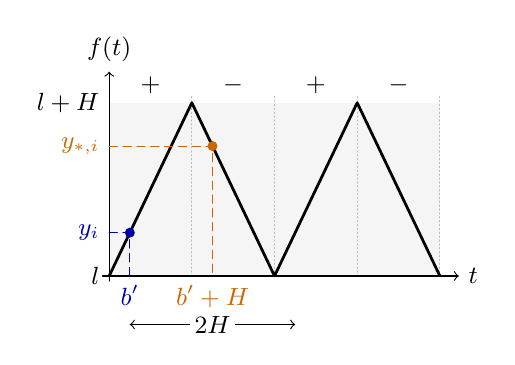
\begin{tikzpicture}[x=1.05cm,y=2.2cm,font=\small,
  line cap=round,line join=round]
  \path[fill=gray!8] (0,0) rectangle (4,1);
  \foreach \x in {0,1,2,3,4}
    \draw[gray!55,densely dotted] (\x,0) -- (\x,1.04);
  \draw[->] (-.08,0) -- (4.23,0) node[right] {$t$};
  \draw[->] (0,-.03) -- (0,1.18) node[above] {$f(t)$};
  \draw[line width=1pt] (0,0) -- (1,1) -- (2,0) -- (3,1) -- (4,0);
  \node[left] at (0,0) {$l$};
  \node[left] at (0,1) {$l+H$};
  \draw[blue!65!black,densely dashed] (0,.25) -- (.25,.25) -- (.25,0);
  \draw[orange!80!black,densely dashed] (0,.75) -- (1.25,.75) -- (1.25,0);
  \fill[blue!65!black] (.25,.25) circle (1.8pt);
  \fill[orange!80!black] (1.25,.75) circle (1.8pt);
  \node[left,text=blue!65!black] at (0,.25) {$y_i$};
  \node[left,text=orange!80!black] at (0,.75) {$y_{*,i}$};
  \node[below,text=blue!65!black] at (.25,0) {$b'$};
  \node[below,text=orange!80!black] at (1.25,0) {$b'+H$};
  \draw[<->] (.25,-.28) -- (2.25,-.28)
    node[midway,fill=white,inner sep=1.5pt] {$2H$};
  \foreach \x/\sign in {.5/+,1.5/-,2.5/+,3.5/-}
    \node at (\x,1.1) {$\sign$};
\end{tikzpicture}
\par\smallskip
{\small
$\displaystyle f(t+H)=2l+H-f(t),$\par
$\displaystyle y_i+y_{*,i}=2l+H.$\par\smallskip
The signs record the alternating\par orientations of successive cells.}
\end{minipage}\hfill
\begin{minipage}[t]{0.54\linewidth}
\centering
\textbf{(b) One successful column}\par\smallskip
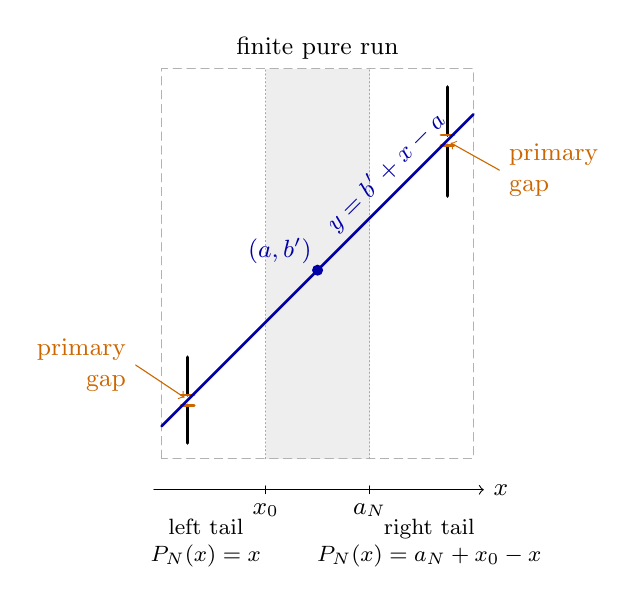
\begin{tikzpicture}[x=.33cm,y=.33cm,font=\small,
  line cap=round,line join=round]
  \path[fill=gray!13] (0,-7) rectangle (4,8);
  \draw[gray!60,densely dashed] (-4,-7) rectangle (8,8);
  \node[above,align=center] at (2,8) {finite pure run};
  \draw[gray!70,densely dotted] (0,-7) -- (0,8);
  \draw[gray!70,densely dotted] (4,-7) -- (4,8);
  \draw[line width=1.3pt] (-3,-6.4) -- (-3,-4.95);
  \draw[line width=1.3pt] (-3,-4.55) -- (-3,-3.1);
  \draw[line width=1.3pt] (7,3.1) -- (7,5.05);
  \draw[line width=1.3pt] (7,5.45) -- (7,7.3);
  \draw[orange!80!black,line width=1pt] (-3.25,-4.95) -- (-2.75,-4.95);
  \draw[orange!80!black,line width=1pt] (-3.25,-4.55) -- (-2.75,-4.55);
  \draw[orange!80!black,line width=1pt] (6.75,5.05) -- (7.25,5.05);
  \draw[orange!80!black,line width=1pt] (6.75,5.45) -- (7.25,5.45);
  \draw[blue!65!black,line width=1pt] (-4,-5.75) -- (8,6.25);
  \fill[blue!65!black] (2,.25) circle (2pt);
  \node[above left,text=blue!65!black,inner sep=2pt] at (2,.25) {$(a,b')$};
  \node[rotate=45,above,text=blue!65!black,inner sep=3pt]
    at (5.2,3.45) {$y=b'+x-a$};
  \draw[orange!80!black,->] (-5,-3.4) -- (-3.12,-4.65);
  \node[left,align=right,text=orange!80!black] at (-5,-3.4)
    {primary\\gap};
  \draw[orange!80!black,->] (9,4.1) -- (7.12,5.15);
  \node[right,align=left,text=orange!80!black] at (9,4.1)
    {primary\\gap};
  \draw[->] (-4.3,-8.2) -- (8.4,-8.2) node[right] {$x$};
  \draw (0,-8.05) -- (0,-8.35) node[below] {$x_0$};
  \draw (4,-8.05) -- (4,-8.35) node[below] {$a_N$};
  \node[align=center,font=\footnotesize] at (-2.3,-10.25)
    {left tail\\$P_N(x)=x$};
  \node[align=center,font=\footnotesize] at (6.3,-10.25)
    {right tail\\$P_N(x)=a_N+x_0-x$};
\end{tikzpicture}
\par\smallskip
{\small
$\displaystyle a\equiv X_*-H+O(\gamma)\pmod{2H}.$\par
Shading marks the central interval, whose image\par
$P_N([x_0,a_N])\subset[x_0-2H,x_0+v]$ is wall-free.}
\end{minipage}
\caption{The two coordinate projections in the final reflection construction.
Write $l=l_i$ and $H=H_i$.
Panel (a) shows the triangular projection to the original marker cell;
shifting a marker ordinate by an odd multiple of $H$ brings its projection
to the anchor height. In panel (b), only the tail-wall portions crossed by
one successful probe line are shown. At either tail wall $x_w$, the
congruence $x_w-a\equiv H+O(\gamma)\pmod{2H}$ places
$f(b'+x_w-a)$ inside a primary gap around $y_{*,i}$. The central
interval has no vertical-wall preimage. The pure run extends beyond the
line's passage through the finite horizontal support, so horizontal
solids are avoided as well. Gap-center crossings and distances are
schematic; the actual $O(\gamma)$ offsets fit within the primary openings.
Secondary gaps make the later fold cuts vacant and are not used for this
diagonal clearance.}
\label{fig:reflection-template-projections}
\end{figure}


Apply the vertical schedule for label $i$ only in word leaves
whose chosen majority label is $i$. All target copies lie on the
retained side of each such vertical fold. Their count doubles
there, while that child's weight is multiplied by $1/2$; their
expected count is therefore unchanged. Minority labels in the
other children are not discarded from the inequality: their total
expected count was already included in the unusable count of
Lemma~\ref{calc:word-purification}. Bad columns cost at most their
fraction times the expected count of the target label, which is
at most one. By choosing the run error and the column error each
less than $\varepsilon/4$, we obtain, for each original marker,
an expected favorable inventory of at least $1-\varepsilon/2$,
apart from coincidences of diagonal projections, addressed next.

\subsubsection{Vacant cuts, stability, and finite extraction}

The word and column constructions have produced the required favorable
inventory. It remains to realize their folds with vacant cuts, keep
the local source routes intact, and extract the favorable copies.
Only after these finite operations are fixed will we choose common
buffers and round to the lattice.

There are only finitely many cuts and copies in the tree just
constructed. Perturb their axis-cut coordinates by sufficiently
small fixed amounts. All successful primary-gap crossings and
pure-run buffers persist. We may require that no cut contain an
endpoint, marked feature, probe, or straight solid segment, and
that distinct insertion copies in any one leaf have distinct
diagonal-time projections $x-y$. To justify the last generic
choice, each copy coordinate is affine in the original coordinates
and in its ancestral cut coordinates. For two different reflection
histories, use the last cut at which the copy histories differ:
its coefficient in their coordinate difference is nonzero, and
subsequent common reflections preserve nonzero dependence.
Thus a coincidence of their diagonal projections is a proper
affine equation in the cuts. If their histories are the same but
their original markers differ, a possible coincidence reduces to
one of the two excluded axis-diagonal equalities for the original
probes. Avoiding finitely many proper affine equations is possible
in every open perturbation neighborhood. The same reasoning
avoids the finitely many incidences of cuts with tips and marked
features. After this perturbation all the retained favorable
copies have slabs avoiding the other insertion boxes as well.

At each transverse intersection of a cut with a solid, insert a
secondary gap at its preimage on the original wall. The generic
choice has kept every such preimage away from original marks,
corners, and primary-gap tips. There are only finitely many distinct
preimages. Merge repeated locations, and take their gap widths
small enough that their neighborhoods are pairwise disjoint and
avoid the protected features. In the reflected copies these gaps
make each prescribed axis cut vacant, with a positive margin. They
only remove solids, so cannot spoil any favorable slab. Source
strings crossing a cut do not constitute solids: their continuous
flux joins are the finite identities in
Proposition~\ref{prop:finite-extraction}. No probabilistic estimate
is being used to make a cut vacant.

We also track the local routing condition at the probes. An axis fold
restricts the diagram to one side and reflects it into the other;
because its cut has positive distance from every probe box, each
surviving box and its arriving prefix are copied intact. No foreign
chain enters a copied box. Any transverse flux join needed at the
cut is made within a vacant margin disjoint from all these boxes.
At a diagonal extraction, choose both the band and its spare routing
margins away from every other box, using their distinct diagonal
projections. Proposition~\ref{prop:finite-extraction} then alters only
the extracted box and these clear margins; all remaining boxes and
their prefixes are copied intact into the two norm diagrams. Induction
therefore preserves the chain-free neighborhood hypothesis for every
later extraction. In particular, this construction never reroutes a
diagonal chain across an unrelated source.

We now apply Lemma~\ref{lem:calc-median-extraction} to the
favorable inventory. The extraction bands contain no other marked
data, as required by Proposition~\ref{prop:finite-extraction}.
Since the preliminary tree has finitely many leaves, a common
finite depth makes their total expected residual favorable count
less than $\varepsilon/2$. Every extracted tagged marker is counted
once, and all other splits preserve tagged counts in half-average.
Combining this residual bound with the favorable inventory above
proves the extracted-count assertion.

Every tagged background feature, excluding all probe insertions,
is intact on one side of every cut and outside every removed middle band.
The two children therefore preserve its expected count. In either
individual child, each retained copy is paired with its mirror,
whose reflection parity is opposite. There was at least one
whole-word end fold, and every subsequent fold or norm split has
the same pairing property. Hence the terminal expected count of
each such feature is one, divided equally between its two
reflection parities. This also explains why the feature count
cannot be replaced by an estimate on arbitrary untracked state
norms.

All inequalities expressing separation in this finite successful
inventory are strict. Holding its chosen cuts and secondary-gap
locations fixed, they remain valid in a neighborhood of the
initial probe pair. A compact eligible set therefore admits a
finite cover by such neighborhoods and their templates. Take the
union of the finitely many secondary-gap locations, merging
coincident locations, and use a common sufficiently small positive
width. The additional vacancies only improve the clearances in
each template.  Shrink the covering neighborhoods to compact
subneighborhoods that still cover the eligible set.  For each
original tip, protected mark, or endpoint, take the minimum of its
strict clearances over every copy in these finite templates and
over every probe pair in the corresponding compact neighborhood.
These clearances include foreign solids and features, all probe
boxes, and every cut, extraction, and rerouting margin.  A smaller
buffered support at the original feature, transported unchanged to
all its copies, is therefore safe throughout the tree.  In
particular its radius does not depend on the actual probe pair.
Finally, round cut lines and gap ends to vertex
lines. Each error is $O(n^{-1})$, and only finitely many reflections
are involved. Thus the total displacement is $O(n^{-1})$ with a
template-dependent constant, smaller than every fixed clearance
for all sufficiently large $n$. The same observation covers all
bounded-mesh shifts of the original data and the local two-step
stencils. This proves Lemma~\ref{lem:reflection-templates}.
\end{proof}
